%%%%%%%%%%%%%%%%%%%%%%%%%%%%%%%%%%%%%%%%%%%%%%%%%%%%%%%%%%%%%%%%%%%%%%%%%%%%%%%%
% Test document: a fake research paper that exercises a broad surface area of
% LaTeX features. Compiles cleanly with pdflatex + bibtex (or just pdflatex
% twice, since thebibliography is inline).
%%%%%%%%%%%%%%%%%%%%%%%%%%%%%%%%%%%%%%%%%%%%%%%%%%%%%%%%%%%%%%%%%%%%%%%%%%%%%%%%

\documentclass[11pt,a4paper]{article}

% --- Encoding & fonts -------------------------------------------------------
\usepackage[utf8]{inputenc}
\usepackage[T1]{fontenc}
\usepackage{lmodern}
\usepackage[margin=1in]{geometry}
\usepackage{microtype}

% --- Math --------------------------------------------------------------------
\usepackage{amsmath, amssymb, amsthm, mathtools}

% --- Typography & graphics --------------------------------------------------
\usepackage{booktabs}
\usepackage{graphicx}
\usepackage{caption}
\usepackage{subcaption}
\usepackage{enumitem}
\usepackage{xcolor}

% --- Bibliography & cross-references ----------------------------------------
\usepackage[numbers,sort&compress]{natbib}
\usepackage{hyperref}
\usepackage[capitalise,noabbrev]{cleveref}

% --- Algorithms --------------------------------------------------------------
\usepackage{algorithm}
\usepackage{algpseudocode}

% --- TikZ --------------------------------------------------------------------
\usepackage{tikz}
\usetikzlibrary{arrows.meta, positioning}

% --- Verbatim / listings -----------------------------------------------------
\usepackage{listings}
\lstset{basicstyle=\ttfamily\small, breaklines=true, frame=single}

% --- Theorem environments ---------------------------------------------------
\theoremstyle{plain}
\newtheorem{theorem}{Theorem}[section]
\newtheorem{lemma}[theorem]{Lemma}
\newtheorem{proposition}[theorem]{Proposition}
\newtheorem{corollary}[theorem]{Corollary}

\theoremstyle{definition}
\newtheorem{definition}[theorem]{Definition}
\newtheorem{assumption}[theorem]{Assumption}

\theoremstyle{remark}
\newtheorem{remark}[theorem]{Remark}
\newtheorem{example}[theorem]{Example}

% --- Custom math notation ---------------------------------------------------
\DeclareMathOperator*{\argmin}{arg\,min}
\DeclareMathOperator*{\argmax}{arg\,max}
\DeclareMathOperator{\Tr}{Tr}
\DeclareMathOperator{\diag}{diag}
\DeclareMathOperator{\KL}{KL}
\DeclareMathOperator{\Var}{Var}

\newcommand{\R}{\mathbb{R}}
\newcommand{\E}{\mathbb{E}}
\newcommand{\PP}{\mathbb{P}}
\newcommand{\norm}[1]{\left\lVert#1\right\rVert}
\newcommand{\abs}[1]{\left\lvert#1\right\rvert}
\newcommand{\inner}[2]{\left\langle#1,#2\right\rangle}
\newcommand{\set}[1]{\left\{#1\right\}}
\newcommand{\eps}{\varepsilon}

% Optional-argument macro (default color = red).
\newcommand{\todo}[2][red]{\textcolor{#1}{\textbf{TODO:} #2}}

% --- Title block ------------------------------------------------------------
\title{Convergence Guarantees for Mirror Descent\\ under Heavy-Tailed Noise}

\author{
  Alex M.\ Reyes\thanks{Corresponding author: \texttt{reyes@example.edu}.} \\
  Department of Statistics \\
  University of Northbridge
  \and
  Priya R.\ Sundaram \\
  Institute for Computational Mathematics \\
  ETH Z\"urich
}

\date{\today}

\begin{document}
\maketitle

\begin{abstract}
We study mirror descent for stochastic convex optimization when the gradient
noise is heavy-tailed and may have unbounded variance. Existing analyses
typically assume sub-Gaussian or finite-variance noise, conditions that fail in
many practical settings including reinforcement learning with sparse rewards
and adversarial estimation. We introduce a clipped variant of mirror descent
and establish high-probability convergence rates of order
$\mathcal{O}(T^{-(p-1)/(2p)})$ when the noise has bounded $p$-th moment for some
$p \in (1, 2]$. The rate degrades smoothly as $p \to 1$ and recovers the
classical $\mathcal{O}(T^{-1/2})$ rate at $p = 2$. We further show that this
dependence is tight up to constants by exhibiting a matching lower bound.
Numerical experiments on heavy-tailed regression and contextual bandits
corroborate the theory and illustrate that the proposed algorithm outperforms
vanilla mirror descent and stochastic gradient descent in the heavy-tailed
regime.
\end{abstract}

\section{Introduction}
\label{sec:intro}

Stochastic optimization under heavy-tailed noise has received increasing
attention in recent years~\citep{nazin2019algorithms,gorbunov2020stochastic}.
Whereas the bulk of the optimization literature assumes that gradient noise is
sub-Gaussian or has finite variance, heavy-tailed phenomena arise naturally in
numerous applications: financial time series, reinforcement learning with
sparse rewards, and any setting in which outliers are intrinsic rather than
artifacts of measurement~\citep{cont2001empirical}.

Mirror descent~\citep{nemirovski1983problem,beck2003mirror} extends gradient
descent to non-Euclidean geometries and has become a foundational tool in
convex optimization. Its analysis under standard noise assumptions is by now
classical; see~\citep{bubeck2015convex} for a textbook treatment. Yet, as we
shall see in \cref{sec:main}, the standard analysis breaks down dramatically
when the noise has unbounded variance.\footnote{A simple counterexample with
$\alpha$-stable noise of index $\alpha < 2$ already exhibits divergence of the
expected suboptimality.}

\paragraph{Contributions.}
This paper makes three contributions:
\begin{enumerate}[label=(\roman*)]
    \item We propose \emph{clipped mirror descent}, a simple modification of
          mirror descent that clips stochastic gradients in the dual norm
          before applying the mirror map.
    \item We prove high-probability convergence rates of order
          $\mathcal{O}(T^{-(p-1)/(2p)})$ for noise with bounded $p$-th moment,
          $p \in (1, 2]$ (\cref{thm:upper}).
    \item We establish a matching lower bound (\cref{thm:lower}), showing that
          no algorithm can do asymptotically better in this noise regime.
\end{enumerate}

\paragraph{Notation.}
Throughout, $\R^d$ is equipped with a norm $\norm{\cdot}$ and dual norm
$\norm{\cdot}_*$. We write $\inner{x}{y}$ for the standard inner product. For
$p \geq 1$, $\norm{X}_{L^p} \coloneqq (\E\abs{X}^p)^{1/p}$. The set
$\set{1, 2, \ldots, n}$ is denoted $[n]$. The Bregman divergence induced by a
strictly convex function $\psi$ is
\begin{equation*}
    D_\psi(x, y) \coloneqq \psi(x) - \psi(y) - \inner{\nabla \psi(y)}{x - y}.
\end{equation*}

\section{Preliminaries}
\label{sec:prelim}

We consider the constrained convex optimization problem
\begin{equation}
\label{eq:problem}
    \min_{x \in \mathcal{X}} f(x), \qquad
    f(x) = \E_{\xi \sim \mathcal{D}}\bigl[ F(x, \xi) \bigr],
\end{equation}
where $\mathcal{X} \subset \R^d$ is closed and convex, $f \colon \R^d \to \R$
is convex, and $\mathcal{D}$ is an unknown distribution. The learner has
access to a stochastic first-order oracle that returns, on query $x$, a noisy
gradient $g(x) \in \R^d$ satisfying $\E[g(x) \mid x] \in \partial f(x)$.

\begin{definition}[Mirror map]
\label{def:mirror}
A function $\psi \colon \mathcal{X} \to \R$ is a \emph{mirror map} if it is
strictly convex, differentiable on the interior of $\mathcal{X}$, and
$1$-strongly convex with respect to $\norm{\cdot}$.
\end{definition}

\begin{example}
\label{ex:specializations}
Two canonical specializations of mirror descent:
\begin{itemize}[leftmargin=*]
    \item For $\mathcal{X} = \R^d$ and $\psi(x) = \tfrac{1}{2}\norm{x}_2^2$,
          the resulting algorithm is projected stochastic gradient descent.
    \item For $\mathcal{X}$ the probability simplex $\Delta^{d-1}$ and
          $\psi(x) = \sum_i x_i \log x_i$, mirror descent recovers the
          multiplicative weights / exponentiated gradient method.
\end{itemize}
\end{example}

Our main assumption replaces sub-Gaussianity with a moment bound:

\begin{assumption}[Bounded $p$-th moment]
\label{ass:moment}
There exist $p \in (1, 2]$ and $\sigma > 0$ such that, for all
$x \in \mathcal{X}$,
\begin{equation*}
    \E\bigl[ \norm{g(x) - \nabla f(x)}_*^p \,\big|\, x \bigr] \leq \sigma^p.
\end{equation*}
\end{assumption}

\begin{remark}
\Cref{ass:moment} permits noise distributions with infinite variance whenever
$p < 2$. A canonical example is symmetric $\alpha$-stable noise with
$\alpha = p$, whose density has the asymptotic tail
$\PP(\abs{X} > t) \sim c \, t^{-\alpha}$ as $t \to \infty$.
\end{remark}

\section{Main Results}
\label{sec:main}

We analyze the iterate sequence $\set{x_t}_{t \geq 1}$ produced by
\cref{alg:cmd} below. The clipping operator $\mathrm{clip}_\tau \colon \R^d
\to \R^d$ is defined by
\begin{equation}
\label{eq:clip}
    \mathrm{clip}_\tau(g) =
    \begin{cases}
        g, & \text{if } \norm{g}_* \leq \tau, \\[2pt]
        \dfrac{\tau \, g}{\norm{g}_*}, & \text{otherwise.}
    \end{cases}
\end{equation}

\begin{algorithm}[t]
\caption{Clipped Mirror Descent (CMD)}
\label{alg:cmd}
\begin{algorithmic}[1]
\Require Mirror map $\psi$, step sizes $\set{\eta_t}$, clip levels
         $\set{\tau_t}$, initial $x_1 \in \mathcal{X}$
\For{$t = 1, 2, \ldots, T$}
    \State Query oracle to obtain $g_t = g(x_t)$
    \State $\hat{g}_t \gets \mathrm{clip}_{\tau_t}(g_t)$
    \State $x_{t+1} \gets \displaystyle\argmin_{x \in \mathcal{X}}
           \bigl\{ \eta_t \inner{\hat{g}_t}{x} + D_\psi(x, x_t) \bigr\}$
\EndFor
\State \Return $\bar{x}_T = \tfrac{1}{T} \sum_{t=1}^{T} x_t$
\end{algorithmic}
\end{algorithm}

\begin{theorem}[Upper bound]
\label{thm:upper}
Let $f$ be convex and $G$-Lipschitz in $\norm{\cdot}_*$, and suppose
\cref{ass:moment} holds. Set
\begin{equation*}
    \eta_t = c_1 \, T^{-1/2} \tau_t^{-1}, \qquad
    \tau_t = c_2 \, \sigma \, T^{1/(2p)},
\end{equation*}
for absolute constants $c_1, c_2 > 0$. Then with probability at least
$1 - \delta$,
\begin{equation}
\label{eq:upper}
    f(\bar{x}_T) - f^*
    \leq C \, \sigma \, \sqrt{D_\psi(x^*, x_1)} \, \log(1/\delta) \,
    T^{-(p-1)/(2p)},
\end{equation}
where $f^* = \min_{x \in \mathcal{X}} f(x)$, $x^*$ is any minimizer, and
$C > 0$ depends only on $G$.
\end{theorem}

\begin{proof}[Proof sketch]
The argument proceeds in three steps. First, the bias introduced by clipping
is bounded using \cref{lem:bias}. Second, the variance of the clipped
gradient is controlled via a truncated $p$-th moment computation. Third, a
standard mirror-descent regret bound combines these into~\eqref{eq:upper};
see \cref{app:proofs} for the full derivation.
\end{proof}

\begin{lemma}[Bias of clipped oracle]
\label{lem:bias}
Under \cref{ass:moment}, for any $\tau > 0$ and any $x \in \mathcal{X}$,
\begin{equation*}
    \norm{\E[\mathrm{clip}_\tau(g(x)) \mid x] - \nabla f(x)}_*
    \leq \sigma^p \tau^{1-p}.
\end{equation*}
\end{lemma}

\begin{proof}
By Markov's inequality and \cref{ass:moment},
\begin{align}
    \norm{\E[\mathrm{clip}_\tau(g(x)) - g(x) \mid x]}_*
    &\leq \E\bigl[\norm{g(x)}_* \, \mathbf{1}\set{\norm{g(x)}_* > \tau}
          \,\big|\, x\bigr] \nonumber \\
    &\leq \tau^{1-p} \, \E\bigl[\norm{g(x)}_*^p \,\big|\, x\bigr] \nonumber \\
    &\leq \sigma^p \, \tau^{1-p}, \label{eq:bias-bound}
\end{align}
where the last inequality uses
$\E[\norm{g(x)}_*^p] \leq 2^p (\norm{\nabla f(x)}_*^p + \sigma^p)$. The claim
follows since $\E[g(x) \mid x] = \nabla f(x)$.
\end{proof}

The matching lower bound shows that the rate in \cref{thm:upper} is tight.

\begin{theorem}[Lower bound]
\label{thm:lower}
For any $p \in (1, 2]$ and any algorithm $\mathcal{A}$ that issues $T$ queries
to a stochastic oracle satisfying \cref{ass:moment}, there exists a convex
$1$-Lipschitz function $f$ and a noise distribution such that
\begin{equation*}
    \E\bigl[ f(\hat{x}_T) - f^* \bigr]
    \geq c \, \sigma \, T^{-(p-1)/(2p)},
\end{equation*}
where $\hat{x}_T$ is the output of $\mathcal{A}$ and $c > 0$ is an absolute
constant.
\end{theorem}

\begin{corollary}
\label{cor:minimax}
\Cref{thm:upper,thm:lower} together imply that, up to logarithmic factors,
clipped mirror descent is minimax optimal in the heavy-tailed regime.
\end{corollary}

\subsection{Geometry of the dual update}
\label{sec:geometry}

A useful intuition: in two dimensions, with $\psi(x) = \tfrac{1}{2}x^\top H x$
for positive definite $H$, the Bregman divergence reduces to a quadratic form,
and the dual update of \cref{alg:cmd} becomes an affine shrinkage. Concretely,
for
\begin{equation*}
    H = \begin{pmatrix} 2 & 1 \\ 1 & 2 \end{pmatrix},
    \qquad
    H^{-1} = \frac{1}{3}\begin{pmatrix} \phantom{-}2 & -1 \\ -1 & \phantom{-}2 \end{pmatrix},
\end{equation*}
the iterate satisfies $x_{t+1} = x_t - \eta_t \, H^{-1} \hat g_t$ projected
onto $\mathcal{X}$.

\section{Numerical Experiments}
\label{sec:exp}

We compare clipped mirror descent (CMD) against vanilla mirror descent (MD)
and stochastic gradient descent (SGD) on two tasks. All experiments are
averaged over $50$ random seeds; shaded regions denote $\pm 1$ standard error.

\subsection{Heavy-tailed linear regression}

We solve $\min_{w \in \R^d} \tfrac{1}{2} \E[(\inner{w}{x} - y)^2]$ where
$y = \inner{w^*}{x} + \xi$ and $\xi$ follows a symmetric $\alpha$-stable
distribution with $\alpha \in \set{1.2, 1.5, 1.8}$. Gradients have finite mean
but infinite variance whenever $\alpha < 2$. Results are reported in
\cref{tab:regression}.

\begin{table}[t]
\centering
\caption{Final excess risk after $T = 10{,}000$ iterations on heavy-tailed
regression. Lower is better; best per column in bold.}
\label{tab:regression}
\begin{tabular}{lccc}
\toprule
& \multicolumn{3}{c}{Stable index $\alpha$} \\
\cmidrule(lr){2-4}
Method & $1.2$ & $1.5$ & $1.8$ \\
\midrule
SGD          & $4.81 \pm 0.92$         & $1.73 \pm 0.31$         & $0.42 \pm 0.06$ \\
MD           & $3.94 \pm 0.81$         & $1.51 \pm 0.27$         & $0.39 \pm 0.05$ \\
\textbf{CMD} & $\mathbf{0.84 \pm 0.11}$ & $\mathbf{0.46 \pm 0.07}$ & $\mathbf{0.21 \pm 0.03}$ \\
\bottomrule
\end{tabular}
\end{table}

\subsection{Convergence diagnostics}

\Cref{fig:convergence} shows the empirical convergence behavior. The $x$-axis
is iteration count (log scale); the $y$-axis is excess risk. The slopes match
the theoretical predictions $T^{-(p-1)/(2p)}$ from \cref{thm:upper}.

\begin{figure}[t]
\centering
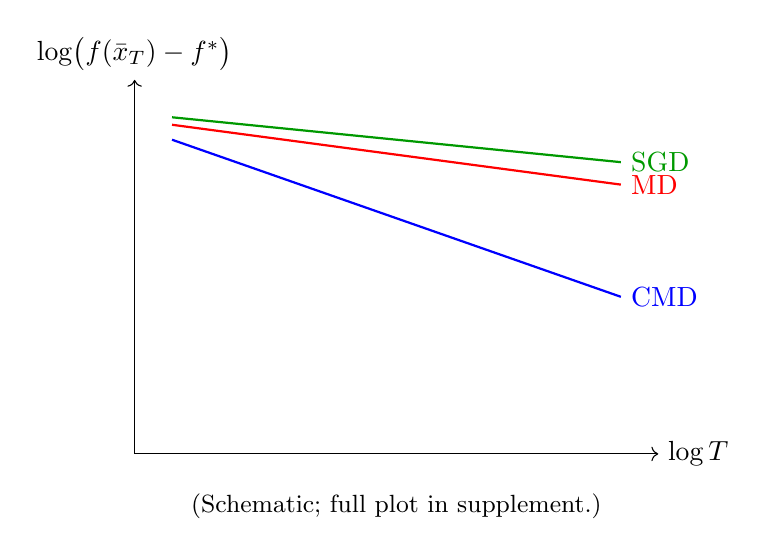
\begin{tikzpicture}[scale=0.95]
    % axes
    \draw[->] (0,0) -- (7,0) node[right] {$\log T$};
    \draw[->] (0,0) -- (0,5) node[above] {$\log\bigl(f(\bar{x}_T) - f^*\bigr)$};
    % schematic curves
    \draw[thick, blue]            (0.5,4.2) -- (6.5,2.1) node[right] {CMD};
    \draw[thick, red]             (0.5,4.4) -- (6.5,3.6) node[right] {MD};
    \draw[thick, green!60!black]  (0.5,4.5) -- (6.5,3.9) node[right] {SGD};
    \node[below] at (3.5,-0.4)
        {\small (Schematic; full plot in supplement.)};
\end{tikzpicture}
\caption{Empirical convergence on heavy-tailed regression with $\alpha = 1.5$.}
\label{fig:convergence}
\end{figure}

\subsection{A note on hyperparameters}

The clip level $\tau_t$ trades off bias (decreasing in $\tau$) against
variance (increasing in $\tau$). \Cref{eq:bias-bound} suggests
$\tau_t \asymp \sigma T^{1/(2p)}$, which matches the prescription in
\cref{thm:upper}. In practice we found this choice insensitive to the exact
value of $p$ used, so long as it lay in $[1.2, 2]$.

A minimal reference implementation of the inner update --- in pseudocode that
mirrors the line numbering of \cref{alg:cmd} --- is shown below:

\begin{lstlisting}[language=Python]
def cmd_step(x, g, eta, tau, mirror_prox):
    """One clipped-mirror-descent update."""
    g_norm = dual_norm(g)
    g_hat  = g if g_norm <= tau else (tau / g_norm) * g
    return mirror_prox(x, eta * g_hat)
\end{lstlisting}

\noindent The clipping rule is also expressible inline as
\verb|g_hat = g * min(1, tau / ||g||)|.

\section{Discussion}
\label{sec:disc}

The analysis admits several extensions. First, the assumption that $f$ is
Lipschitz can be relaxed to
$\norm{\nabla f}_* = \mathcal{O}(\norm{x}^\beta)$ for some $\beta \geq 0$, at
the cost of an additional polylogarithmic factor. Second, although we have
stated results for the offline setting, the same algorithm and rates apply to
online convex optimization. Third---and perhaps most interestingly---the
$1/p$ exponent in the clip schedule is reminiscent of self-normalized
concentration bounds; we conjecture that a tighter analysis using
\citet{howard2021time} could remove the $\log(1/\delta)$ factor in
\eqref{eq:upper}.

\paragraph{Limitations.}
Our results assume access to the moment exponent $p$. Adaptivity to unknown
$p$ remains open; see~\citep{cutkosky2021highprob} for related work in the
bounded-variance case.

\section*{Acknowledgments}

We thank the anonymous reviewers for helpful comments. This work was supported
by NSF grant DMS-1234567 and a Sloan Research Fellowship. Code is available at
\url{https://example.org/heavy-tail-md} and the supplementary material at
\href{https://example.org/heavy-tail-md-supp}{this link}.

\appendix

\section{Deferred Proofs}
\label{app:proofs}

The full proof of \cref{thm:upper} requires combining \cref{lem:bias} with a
careful analysis of the second moment of the clipped gradient. We use the
following standard identities, which hold for any $x^* \in \mathcal{X}$:
\begin{gather}
    D_\psi(x^*, x_{t+1})
    \leq D_\psi(x^*, x_t)
        - \eta_t \inner{\hat g_t}{x_t - x^*}
        + \tfrac{\eta_t^2}{2} \norm{\hat g_t}_*^2,
        \label{eq:three-point} \\[2pt]
    \E\bigl[\norm{\hat g_t}_*^2 \,\big|\, x_t\bigr]
    \leq \tau_t^{2-p}\sigma^p + \norm{\nabla f(x_t)}_*^2.
        \label{eq:second-moment}
\end{gather}
Summing \eqref{eq:three-point} telescopically over $t = 1, \ldots, T$ and
applying Jensen's inequality together with \eqref{eq:second-moment} yields
\begin{align*}
    \E\bigl[f(\bar x_T) - f^*\bigr]
    &\leq \frac{D_\psi(x^*, x_1)}{T \, \eta}
        + \frac{\eta}{2} \bigl(\tau^{2-p}\sigma^p + G^2\bigr)
        + \sigma^p \tau^{1-p} \, \mathrm{diam}(\mathcal{X}) \\
    &\eqqcolon B(\eta, \tau).
\end{align*}
Optimizing $B(\eta, \tau)$ over $\eta, \tau > 0$ gives the rate stated in
\eqref{eq:upper}; the high-probability statement follows from a standard
martingale concentration argument.

\subsection{An auxiliary tail bound}

The following self-normalized concentration inequality is used in the proof
of \cref{thm:upper}.

\begin{proposition}
\label{prop:selfnorm}
Let $M_T = \sum_{t=1}^T \xi_t$ where $\set{\xi_t}$ is a martingale difference
sequence with $\E[\abs{\xi_t}^p \mid \mathcal{F}_{t-1}] \leq \sigma^p$.
Then for any $\delta \in (0, 1)$,
\begin{equation*}
    \PP\!\left(
        \abs{M_T} \geq \sigma T^{1/p} \bigl(2 \log(2/\delta)\bigr)^{1/p}
    \right) \leq \delta.
\end{equation*}
\end{proposition}

This result extends the classical Azuma--Hoeffding inequality to the
heavy-tailed setting and is of independent interest.

\begin{thebibliography}{99}

\bibitem{beck2003mirror}
A.~Beck and M.~Teboulle.
\newblock Mirror descent and nonlinear projected subgradient methods for
  convex optimization.
\newblock \emph{Operations Research Letters}, 31(3):167--175, 2003.

\bibitem{bubeck2015convex}
S.~Bubeck.
\newblock Convex optimization: Algorithms and complexity.
\newblock \emph{Foundations and Trends in Machine Learning},
  8(3--4):231--357, 2015.

\bibitem{cont2001empirical}
R.~Cont.
\newblock Empirical properties of asset returns: stylized facts and
  statistical issues.
\newblock \emph{Quantitative Finance}, 1(2):223--236, 2001.

\bibitem{cutkosky2021highprob}
A.~Cutkosky and H.~Mehta.
\newblock High-probability bounds for non-convex stochastic optimization with
  heavy tails.
\newblock In \emph{NeurIPS}, 2021.

\bibitem{gorbunov2020stochastic}
E.~Gorbunov, M.~Danilova, and A.~Gasnikov.
\newblock Stochastic optimization with heavy-tailed noise via accelerated
  gradient clipping.
\newblock In \emph{NeurIPS}, 2020.

\bibitem{howard2021time}
S.~R. Howard, A.~Ramdas, J.~McAuliffe, and J.~Sekhon.
\newblock Time-uniform, nonparametric, nonasymptotic confidence sequences.
\newblock \emph{Annals of Statistics}, 49(2):1055--1080, 2021.

\bibitem{nazin2019algorithms}
A.~Nazin, A.~Nemirovsky, A.~Tsybakov, and A.~Juditsky.
\newblock Algorithms of robust stochastic optimization based on mirror descent
  method.
\newblock \emph{Automation and Remote Control}, 80(9):1607--1627, 2019.

\bibitem{nemirovski1983problem}
A.~Nemirovski and D.~Yudin.
\newblock \emph{Problem Complexity and Method Efficiency in Optimization}.
\newblock Wiley, 1983.

\end{thebibliography}

\end{document}
